% answers.tex —— 2013 年·春季上海卷 · 参考答案与详细解析片段
% 由 tools/generate_projects.py 依来源总账自 2013/2013_数学真题_春季上海_试题.md + 2013/2013_数学真题_春季上海_解析正文.md + 2013/2013_数学真题_春季上海_答案要点.md 生成，勿手改（改源 MD 后重跑）


\begin{answer}
\gksolhead{1}{}

\textbf{题目}：

函数 $y=\log_2(x+2)$ 的定义域是\gkblank{}。

\Needspace{4\baselineskip}
\textbf{解析}

\Needspace{5\baselineskip}
对数的真数必须为正，故
\nopagebreak[4]
\[x+2>0,\]
\Needspace{5\baselineskip}
解得
\nopagebreak[4]
\[x>-2.\]
因此定义域为 $(-2,+\infty)$。

\gkanswer{答案：$(-2,+\infty)$。由真数 $x+2>0$ 得 $x>-2$。}

\end{answer}
\begin{answer}
\gksolhead{2}{}

\textbf{题目}：

方程 $2^x=8$ 的解是\gkblank{}。

\Needspace{4\baselineskip}
\textbf{解析}

\Needspace{5\baselineskip}
把 $8$ 写成以 $2$ 为底的幂：
\nopagebreak[4]
\[2^x=8=2^3.\]
\Needspace{5\baselineskip}
指数函数 $y=2^x$ 在 $\mathbf R$ 上单调，故
\nopagebreak[4]
\[x=3.\]

\gkanswer{答案：$3$。$2^x=8=2^3$，指数函数单调，故 $x=3$。}

\end{answer}
\begin{answer}
\gksolhead{3}{}

\textbf{题目}：

抛物线 $y^2=8x$ 的准线方程是\gkblank{}。

\Needspace{4\baselineskip}
\textbf{解析}

\Needspace{5\baselineskip}
抛物线 $y^2=8x$ 的标准形式为 $y^2=2px$，故
\nopagebreak[4]
\[2p=8,\qquad p=4.\]
\Needspace{5\baselineskip}
其准线为
\nopagebreak[4]
\[x=-\frac p2=-2.\]

\gkanswer{答案：$x=-2$。$y^2=8x$ 中 $2p=8$，准线为 $x=-\dfrac p2=-2$。}

\end{answer}
\begin{answer}
\gksolhead{4}{}

\textbf{题目}：

函数 $y=2\sin x$ 的最小正周期是\gkblank{}。

\Needspace{4\baselineskip}
\textbf{解析}

\Needspace{5\baselineskip}
函数 $y=2\sin x$ 中 $\omega=1$，最小正周期为
\nopagebreak[4]
\[T=\frac{2\pi}{|\omega|}=2\pi.\]

\gkanswer{答案：$2\pi$。$\omega=1$，$T=\dfrac{2\pi}{|\omega|}=2\pi$。}

\end{answer}
\begin{answer}
\gksolhead{5}{}

\textbf{题目}：

已知向量 $\boldsymbol a=(1,k)$，$\boldsymbol b=(9,k-6)$。若 $\boldsymbol a\parallel\boldsymbol b$，则实数 $k=$\gkblank{}。

\Needspace{4\baselineskip}
\textbf{解析}

\Needspace{5\baselineskip}
两向量平行的充要条件是坐标行列式为零：
\nopagebreak[4]
\[\begin{vmatrix}1&k\\9&k-6\end{vmatrix}=0,\]
\Needspace{5\baselineskip}
即
\nopagebreak[4]
\[1\cdot(k-6)-9k=0.\]
\Needspace{5\baselineskip}
整理得
\nopagebreak[4]
\[-8k-6=0,\]
\Needspace{5\baselineskip}
故
\nopagebreak[4]
\[k=-\frac34.\]
此时 $\boldsymbol a=(1,-\tfrac34)$，$\boldsymbol b=(9,-\tfrac{27}4)$，确有 $\boldsymbol b=9\boldsymbol a$。

\gkanswer{答案：$-\dfrac34$。由 $1\cdot(k-6)-9k=0$ 得 $k=-\dfrac34$。}

\end{answer}
\begin{answer}
\gksolhead{6}{}

\textbf{题目}：

函数 $y=4\sin x+3\cos x$ 的最大值是\gkblank{}。

\Needspace{4\baselineskip}
\textbf{解析}

\Needspace{5\baselineskip}
用辅助角公式：
\nopagebreak[4]
\[4\sin x+3\cos x=5\left(\frac45\sin x+\frac35\cos x\right)=5\sin(x+\varphi),\]
\Needspace{5\baselineskip}
其中 $\cos\varphi=\dfrac45$，$\sin\varphi=\dfrac35$。因正弦值不超过 $1$，故最大值为
\nopagebreak[4]
\[5.\]

\gkanswer{答案：$5$。$4\sin x+3\cos x=5\sin(x+\varphi)$，最大值为 $\sqrt{4^2+3^2}=5$。}

\end{answer}
\begin{answer}
\gksolhead{7}{}

\textbf{题目}：

复数 $2+3\mathrm i$（$\mathrm i$ 是虚数单位）的模是\gkblank{}。

\Needspace{4\baselineskip}
\textbf{解析}

\Needspace{5\baselineskip}
复数 $z=2+3\mathrm i$ 的模为
\nopagebreak[4]
\[|z|=\sqrt{2^2+3^2}=\sqrt{13}.\]

\gkanswer{答案：$\sqrt{13}$。$|2+3\mathrm i|=\sqrt{2^2+3^2}=\sqrt{13}$。}

\end{answer}
\begin{answer}
\gksolhead{8}{}

\textbf{题目}：

在 $\triangle ABC$ 中，角 $A$、$B$、$C$ 所对边长分别为 $a$、$b$、$c$，若 $a=5$，$c=8$，$B=60^\circ$，则 $b=$\gkblank{}。

\Needspace{4\baselineskip}
\textbf{解析}

\Needspace{5\baselineskip}
按余弦定理，
\nopagebreak[4]
\[b^2=a^2+c^2-2ac\cos B.\]
\Needspace{5\baselineskip}
代入 $a=5$，$c=8$，$B=60^\circ$：
\nopagebreak[4]
\[b^2=25+64-2\cdot5\cdot8\cdot\frac12=89-40=49,\]
\Needspace{5\baselineskip}
故
\nopagebreak[4]
\[b=7.\]

需要说明：原卷第 1 页此题印面作“$a=5$，$b=8$，$B=60^\circ$，则 $b=$”，同句既给出 $b=8$ 又要求 $b$，自相矛盾；只有把第二个已知边读作 $c=8$，才能与官方答案 $7$ 相容。故本稿按 $c=8$ 转录，判定原卷此处为“$c$”误印成“$b$”。

\gkanswer{答案：$7$。由余弦定理 $b^2=5^2+8^2-2\cdot5\cdot8\cos60^\circ=49$；原卷印面“$b=8$”与所求 $b$ 矛盾，应为“$c=8$”。}

\end{answer}
\begin{answer}
\gksolhead{9}{}

\textbf{题目}：

在如图所示的正方体 $ABCD-A_1B_1C_1D_1$ 中，异面直线 $A_1B$ 与 $B_1C$ 所成角的大小为\gkblank{}。
\nopagebreak[4]
\begin{center}% 2013 年春季上海卷第 9 题：正方体 ABCD-A1B1C1D1
% 突出异面直线 A1B 与 B1C；图中透视比例不代表题设尺寸。
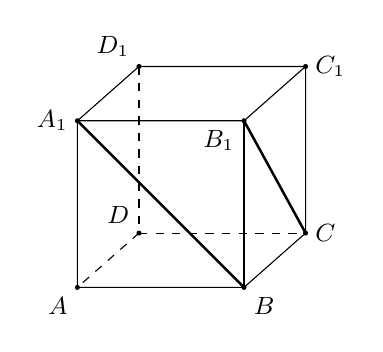
\begin{tikzpicture}[>=stealth, scale=0.92, font=\small]
  \coordinate (A)  at (0,0);
  \coordinate (B)  at (2.30,0);
  \coordinate (C)  at (3.15,0.75);
  \coordinate (D)  at (0.85,0.75);
  \coordinate (A1) at (0,2.30);
  \coordinate (B1) at (2.30,2.30);
  \coordinate (C1) at (3.15,3.05);
  \coordinate (D1) at (0.85,3.05);
  % 可见棱
  \draw (A) -- (B) -- (C) -- (C1) -- (B1) -- (A1) -- cycle;
  \draw (A1) -- (D1) -- (C1);
  \draw (B) -- (B1);
  % 不可见棱
  \draw[dashed] (D1) -- (D);
  \draw[dashed] (D) -- (C);
  \draw[dashed] (D) -- (A);
  % 异面直线 A1B 与 B1C
  \draw[line width=0.9pt] (A1) -- (B);
  \draw[line width=0.9pt] (B1) -- (C);
  % 顶点
  \fill (A) circle (1pt) node[below left] {$A$};
  \fill (B) circle (1pt) node[below right] {$B$};
  \fill (C) circle (1pt) node[right] {$C$};
  \fill (D) circle (1pt) node[above left] {$D$};
  \fill (A1) circle (1pt) node[left] {$A_1$};
  \fill (B1) circle (1pt) node[below left] {$B_1$};
  \fill (C1) circle (1pt) node[right] {$C_1$};
  \fill (D1) circle (1pt) node[above left] {$D_1$};
\end{tikzpicture}
\end{center}
\nopagebreak[4]
\Needspace{4\baselineskip}
\textbf{解析}

\Needspace{5\baselineskip}
设立方体棱长为 $1$，取坐标
\nopagebreak[4]
\[A(0,0,0),\ B(1,0,0),\ C(1,1,0),\ D(0,1,0),\]
\nopagebreak[4]
\[A_1(0,0,1),\ B_1(1,0,1),\ C_1(1,1,1),\]
\Needspace{5\baselineskip}
则
\nopagebreak[4]
\[\overrightarrow{A_1B}=(1,0,-1),\qquad \overrightarrow{B_1C}=(0,1,-1).\]
\Needspace{5\baselineskip}
于是
\nopagebreak[4]
\[\overrightarrow{A_1B}\cdot\overrightarrow{B_1C}=0+0+1=1,\]
\nopagebreak[4]
\[|\overrightarrow{A_1B}|=|\overrightarrow{B_1C}|=\sqrt2.\]
\Needspace{5\baselineskip}
设两直线所成角为 $\alpha$，则
\nopagebreak[4]
\[\cos\alpha=\frac{1}{\sqrt2\cdot\sqrt2}=\frac12,\]
\Needspace{5\baselineskip}
故
\nopagebreak[4]
\[\alpha=\frac\pi3.\]

也可取 $A_1B\parallel D_1C$，在 $\triangle B_1CD_1$ 中三边均为面对角线 $\sqrt2$，三角形为等边三角形，故 $\angle B_1CD_1=\dfrac\pi3$。

\gkanswer{答案：$\dfrac\pi3$。$\overrightarrow{A_1B}=(1,0,-1)$，$\overrightarrow{B_1C}=(0,1,-1)$，夹角余弦为 $\dfrac12$。}

\end{answer}
\begin{answer}
\gksolhead{10}{}

\textbf{题目}：

从 $4$ 名男同学和 $6$ 名女同学中随机选取 $3$ 人参加某社团活动，选出的 $3$ 人中男女同学都有的概率为\gkblank{}（结果用数值表示）。

\Needspace{4\baselineskip}
\textbf{解析}

\Needspace{5\baselineskip}
从 $10$ 人中任选 $3$ 人，共有
\nopagebreak[4]
\[\mathrm C_{10}^3=120\]
\Needspace{5\baselineskip}
种选法。用对立事件“$3$ 人全为男生或全为女生”计数：
\nopagebreak[4]
\[\mathrm C_4^3+\mathrm C_6^3=4+20=24.\]
\Needspace{5\baselineskip}
故男女都有的概率为
\nopagebreak[4]
\[1-\frac{24}{120}=1-\frac15=\frac45.\]

\gkanswer{答案：$\dfrac45$。$1-\dfrac{\mathrm C_4^3+\mathrm C_6^3}{\mathrm C_{10}^3}=1-\dfrac{24}{120}=\dfrac45$。}

\end{answer}
\begin{answer}
\gksolhead{11}{}

\textbf{题目}：

若等差数列的前 $6$ 项和为 $23$，前 $9$ 项和为 $57$，则数列的前 $n$ 项和 $S_n=$\gkblank{}。

\Needspace{4\baselineskip}
\textbf{解析}

\Needspace{5\baselineskip}
设首项为 $a_1$，公差为 $d$。由前 $n$ 项和公式得
\nopagebreak[4]
\[\begin{cases}6a_1+15d=23,\\ 9a_1+36d=57.\end{cases}\]
\Needspace{5\baselineskip}
第一式乘 $3$、第二式乘 $2$：
\nopagebreak[4]
\[18a_1+45d=69,\qquad 18a_1+72d=114.\]
\Needspace{5\baselineskip}
相减得
\nopagebreak[4]
\[27d=45,\qquad d=\frac53.\]
\Needspace{5\baselineskip}
代回 $6a_1+15\cdot\dfrac53=23$，即 $6a_1+25=23$，得
\nopagebreak[4]
\[a_1=-\frac13.\]
\Needspace{5\baselineskip}
于是
\nopagebreak[4]
\[S_n=na_1+\frac{n(n-1)}2d
=-\frac n3+\frac{5n(n-1)}6
=\frac{5n^2-7n}{6}.\]

\gkanswer{答案：$\dfrac56n^2-\dfrac76n$。由 $6a_1+15d=23$、$9a_1+36d=57$ 得 $a_1=-\dfrac13$，$d=\dfrac53$。}

\end{answer}
\begin{answer}
\gksolhead{12}{}

\textbf{题目}：

$36$ 的所有正约数之和可按如下方法得到：

\Needspace{5\baselineskip}
因为 $36=2^2\times3^2$，所以 $36$ 的所有正约数之和为

\nopagebreak[4]
\[(1+3+3^2)+(2+2\times3+2\times3^2)+(2^2+2^2\times3+2^2\times3^2)=(1+2+2^2)(1+3+3^2)=91.\]

参照上述方法，可求得 $2000$ 的所有正约数之和为\gkblank{}。

\Needspace{4\baselineskip}
\textbf{解析}

\Needspace{5\baselineskip}
先分解质因数：
\nopagebreak[4]
\[2000=2^4\cdot5^3.\]
\Needspace{5\baselineskip}
仿照题中把各素因子幂的全部搭配相加的做法，所有正约数之和为
\nopagebreak[4]
\[(1+2+2^2+2^3+2^4)(1+5+5^2+5^3).\]
\Needspace{5\baselineskip}
分别求和：
\nopagebreak[4]
\[1+2+4+8+16=31,\qquad 1+5+25+125=156.\]
\Needspace{5\baselineskip}
故
\nopagebreak[4]
\[31\times156=4836.\]

\gkanswer{答案：$4836$。$2000=2^4\cdot5^3$，约数和为 $(1+2+4+8+16)(1+5+25+125)=31\times156$。}

\end{answer}
\begin{answer}
\gksolhead{13}{}

\textbf{题目}：

展开式为 $ad-bc$ 的行列式是\mbox{（　　）}

（A）$\begin{vmatrix}a&b\\d&c\end{vmatrix}$；（B）$\begin{vmatrix}a&c\\b&d\end{vmatrix}$；（C）$\begin{vmatrix}a&d\\b&c\end{vmatrix}$；（D）$\begin{vmatrix}b&a\\d&c\end{vmatrix}$。

\Needspace{4\baselineskip}
\textbf{解析}

\Needspace{5\baselineskip}
二阶行列式的定义是
\nopagebreak[4]
\[\begin{vmatrix}a&b\\c&d\end{vmatrix}=ad-bc.\]
\Needspace{5\baselineskip}
逐项核对：
\nopagebreak[4]
\[\begin{vmatrix}a&b\\d&c\end{vmatrix}=ac-bd,\qquad
\begin{vmatrix}a&c\\b&d\end{vmatrix}=ad-bc,\]
\nopagebreak[4]
\[\begin{vmatrix}a&d\\b&c\end{vmatrix}=ac-bd,\qquad
\begin{vmatrix}b&a\\d&c\end{vmatrix}=bc-ad.\]
只有第二项等于 $ad-bc$。

选 B。

\gkanswer{答案：B。$\begin{vmatrix}a&c\\b&d\end{vmatrix}=ad-bc$。}

\end{answer}
\begin{answer}
\gksolhead{14}{}

\textbf{题目}：

设 $f^{-1}(x)$ 为函数 $f(x)=\sqrt x$ 的反函数，下列结论正确的是\mbox{（　　）}

（A）$f^{-1}(2)=2$；（B）$f^{-1}(2)=4$；（C）$f^{-1}(4)=2$；（D）$f^{-1}(4)=4$。

\Needspace{4\baselineskip}
\textbf{解析}

\Needspace{5\baselineskip}
由 $y=\sqrt x$（$x\geqslant0$，$y\geqslant0$）得 $x=y^2$，故反函数为
\nopagebreak[4]
\[f^{-1}(x)=x^2,\qquad x\geqslant0.\]
\Needspace{5\baselineskip}
于是
\nopagebreak[4]
\[f^{-1}(2)=4,\qquad f^{-1}(4)=16.\]
只有 $f^{-1}(2)=4$ 正确。

选 B。

\gkanswer{答案：B。$f^{-1}(x)=x^2$（$x\geqslant0$），故 $f^{-1}(2)=4$。}

\end{answer}
\begin{answer}
\gksolhead{15}{}

\textbf{题目}：

直线 $2x-3y+1=0$ 的一个方向向量是\mbox{（　　）}

（A）$(2,-3)$；（B）$(2,3)$；（C）$(-3,2)$；（D）$(3,2)$。

\Needspace{4\baselineskip}
\textbf{解析}

\Needspace{5\baselineskip}
直线 $2x-3y+1=0$ 的法向量为 $(2,-3)$，故一个方向向量与之垂直，可取
\nopagebreak[4]
\[(3,2),\]
因为 $2\cdot3+(-3)\cdot2=0$。

选 D。

\gkanswer{答案：D。法向量 $(2,-3)$ 与 $(3,2)$ 垂直，后者是方向向量。}

\end{answer}
\begin{answer}
\gksolhead{16}{}

\textbf{题目}：

函数 $f(x)=x^{-\frac12}$ 的大致图像是\mbox{（　　）}
\nopagebreak[4]
\begin{center}% 2013 年春季上海卷第 16 题：f(x)=x^{-1/2} 的候选图像
% 四个小坐标系按原卷自左至右排列，依次标 (A)(B)(C)(D)。
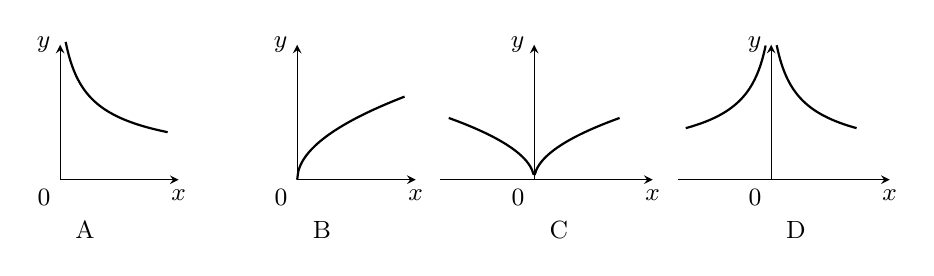
\begin{tikzpicture}[>=stealth, scale=0.70, font=\small]
  % (A) 定义域 x>0，单调递减
  \begin{scope}
    \draw[->] (0,0) -- (2.15,0) node[below] {$x$};
    \draw[->] (0,0) -- (0,2.45) node[left] {$y$};
    \node[below left] at (0,0) {$0$};
    \draw[thick, domain=0.10:1.95, samples=90, smooth]
      plot (\x,{1.25/sqrt(\x+0.15)});
    \node at (0.45,-0.92) {A};
  \end{scope}
  % (B) 过原点，单调递增
  \begin{scope}[xshift=4.30cm]
    \draw[->] (0,0) -- (2.15,0) node[below] {$x$};
    \draw[->] (0,0) -- (0,2.45) node[left] {$y$};
    \node[below left] at (0,0) {$0$};
    \draw[thick, domain=0:1.95, samples=90, smooth]
      plot (\x,{1.08*sqrt(\x)});
    \node at (0.45,-0.92) {B};
  \end{scope}
  % (C) 关于 y 轴对称，原点处取最小值
  \begin{scope}[xshift=8.60cm]
    \draw[->] (-1.70,0) -- (2.15,0) node[below] {$x$};
    \draw[->] (0,0) -- (0,2.45) node[left] {$y$};
    \node[below left] at (0,0) {$0$};
    \draw[thick, domain=-1.55:1.55, samples=120, smooth]
      plot (\x,{0.90*sqrt(abs(\x))});
    \node at (0.45,-0.92) {C};
  \end{scope}
  % (D) 关于 y 轴对称，两侧单调递减
  \begin{scope}[xshift=12.90cm]
    \draw[->] (-1.70,0) -- (2.15,0) node[below] {$x$};
    \draw[->] (0,0) -- (0,2.45) node[left] {$y$};
    \node[below left] at (0,0) {$0$};
    \draw[thick, domain=0.10:1.55, samples=90, smooth]
      plot (\x,{1.22/sqrt(\x+0.15)});
    \draw[thick, domain=-1.55:-0.10, samples=90, smooth]
      plot (\x,{1.22/sqrt(-\x+0.15)});
    \node at (0.45,-0.92) {D};
  \end{scope}
\end{tikzpicture}
\end{center}
\nopagebreak[4]
\Needspace{4\baselineskip}
\textbf{解析}

\Needspace{5\baselineskip}
函数
\nopagebreak[4]
\[f(x)=x^{-\frac12}=\frac1{\sqrt x}\]
的定义域为 $x>0$，且在 $(0,+\infty)$ 上单调递减；当 $x\to0^+$ 时 $f(x)\to+\infty$，当 $x\to+\infty$ 时 $f(x)\to0^+$。

四个候选图中：图 B 单调递增；图 C、D 的图像关于 $y$ 轴对称，定义域含负值；只有图 A 位于第一象限、单调递减并以两坐标轴为渐近线，符合 $f(x)=\dfrac1{\sqrt x}$。

选 A。

\gkanswer{答案：A。$f(x)=\dfrac1{\sqrt x}$ 定义域为 $x>0$ 且单调递减。}

\end{answer}
\begin{answer}
\gksolhead{17}{}

\textbf{题目}：

如果 $a<b<0$，那么下列不等式成立的是\mbox{（　　）}

（A）$\dfrac1a<\dfrac1b$；（B）$ab<b^2$；（C）$-ab<-a^2$；（D）$-\dfrac1a<-\dfrac1b$。

\Needspace{4\baselineskip}
\textbf{解析}

\Needspace{5\baselineskip}
由 $a<b<0$ 知 $|a|>|b|>0$，且
\nopagebreak[4]
\[-\frac1a=\frac1{|a|},\qquad -\frac1b=\frac1{|b|}.\]
\Needspace{5\baselineskip}
因为 $|a|>|b|$，所以
\nopagebreak[4]
\[\frac1{|a|}<\frac1{|b|},\]
\Needspace{5\baselineskip}
即
\nopagebreak[4]
\[-\frac1a<-\frac1b.\]

\Needspace{5\baselineskip}
其余三项均可举反例。取 $a=-2$，$b=-1$：
\nopagebreak[4]
\[\frac1a=-\frac12>-1=\frac1b,\]
故（A）不成立；$ab=2$，$b^2=1$，故（B）不成立；$-ab=-2$，$-a^2=-4$，故（C）不成立。

选 D。

\gkanswer{答案：D。$a<b<0$ 时 $|a|>|b|$，故 $-\dfrac1a=\dfrac1{|a|}<\dfrac1{|b|}=-\dfrac1b$。}

\end{answer}
\begin{answer}
\gksolhead{18}{}

\textbf{题目}：

若复数 $z_1$、$z_2$ 满足 $z_1=\overline{z_2}$，则 $z_1$、$z_2$ 在复数平面上对应的点 $Z_1$、$Z_2$\mbox{（　　）}

（A）关于 $x$ 轴对称；（B）关于 $y$ 轴对称；（C）关于原点对称；（D）关于直线 $y=x$ 对称。

\Needspace{4\baselineskip}
\textbf{解析}

\Needspace{5\baselineskip}
设 $z_2=x+y\mathrm i$（$x,y\in\mathbf R$），则
\nopagebreak[4]
\[z_1=\overline{z_2}=x-y\mathrm i.\]
于是 $Z_1(x,-y)$，$Z_2(x,y)$，两点横坐标相同、纵坐标互为相反数，故关于 $x$ 轴对称。

选 A。

\gkanswer{答案：A。$z_2=x+y\mathrm i$ 时 $z_1=x-y\mathrm i$，两点关于 $x$ 轴对称。}

\end{answer}
\begin{answer}
\gksolhead{19}{}

\textbf{题目}：

$(1+x)^{10}$ 的二项展开式中的一项是\mbox{（　　）}

（A）$45x$；（B）$90x^2$；（C）$120x^3$；（D）$252x^4$。

\Needspace{4\baselineskip}
\textbf{解析}

\Needspace{5\baselineskip}
二项展开式的通项为
\nopagebreak[4]
\[T_{k+1}=\mathrm C_{10}^k x^k,\qquad k=0,1,\dots,10.\]
\Needspace{5\baselineskip}
逐项核对：
\nopagebreak[4]
\[\mathrm C_{10}^1=10,\quad
\mathrm C_{10}^2=45,\quad
\mathrm C_{10}^3=120,\quad
\mathrm C_{10}^4=210.\]
故 $x$、$x^2$、$x^3$、$x^4$ 的系数依次为 $10,45,120,210$。选项中只有 $120x^3$ 是展开式中的一项。

选 C。

\gkanswer{答案：C。$x^3$ 的系数为 $\mathrm C_{10}^3=120$。}

\end{answer}
\begin{answer}
\gksolhead{20}{}

\textbf{题目}：

既是偶函数又在区间 $(0,\pi)$ 上单调递减的函数是\mbox{（　　）}

（A）$y=\sin x$；（B）$y=\cos x$；（C）$y=\sin 2x$；（D）$y=\cos 2x$。

\Needspace{4\baselineskip}
\textbf{解析}

先看奇偶性：$\sin x$、$\sin2x$ 为奇函数，$\cos x$、$\cos2x$ 为偶函数，故只需在 $\cos x$ 与 $\cos2x$ 中比较。

在 $(0,\pi)$ 上，$y=\cos x$ 单调递减；而 $y=\cos2x$ 在 $\left(0,\dfrac\pi2\right)$ 上递减、在 $\left(\dfrac\pi2,\pi\right)$ 上递增，不满足单调递减。

选 B。

\gkanswer{答案：B。$\cos x$ 为偶函数，且在 $(0,\pi)$ 上单调递减。}

\end{answer}
\begin{answer}
\gksolhead{21}{}

\textbf{题目}：

若两个球的表面积之比为 $1:4$，则这两个球的体积之比为\mbox{（　　）}

（A）$1:2$；（B）$1:4$；（C）$1:8$；（D）$1:16$。

\Needspace{4\baselineskip}
\textbf{解析}

\Needspace{5\baselineskip}
两球表面积之比为
\nopagebreak[4]
\[\frac{S_1}{S_2}=\left(\frac{r_1}{r_2}\right)^2=\frac14,\]
\Needspace{5\baselineskip}
故半径之比
\nopagebreak[4]
\[\frac{r_1}{r_2}=\frac12.\]
\Needspace{5\baselineskip}
体积之比为
\nopagebreak[4]
\[\frac{V_1}{V_2}=\left(\frac{r_1}{r_2}\right)^3=\frac18.\]

选 C。

\gkanswer{答案：C。表面积比 $1:4$ 给出半径比 $1:2$，体积比 $1:8$。}

\end{answer}
\begin{answer}
\gksolhead{22}{}

\textbf{题目}：

设全集 $U=\mathbf R$，下列集合运算结果为 $\mathbf R$ 的是\mbox{（　　）}

（A）$\mathbf Z\cup\complement_U\mathbf N$；（B）$\mathbf N\cap\complement_U\mathbf N$；（C）$\complement_U(\complement_U\varnothing)$；（D）$\complement_U\{0\}$。

\Needspace{4\baselineskip}
\textbf{解析}

逐项判断，其中 $\complement_U A$ 表示 $A$ 在 $\mathbf R$ 中的补集。

（A）$\mathbf Z\cup\complement_U\mathbf N$：任一实数或是整数，或不是自然数。非整数的实数都不属于 $\mathbf N$，故属于 $\complement_U\mathbf N$；整数属于 $\mathbf Z$。因此并集为 $\mathbf R$。

（B）$\mathbf N\cap\complement_U\mathbf N=\varnothing$。

（C）$\complement_U(\complement_U\varnothing)=\varnothing$。

（D）$\complement_U\{0\}=\mathbf R\setminus\{0\}\neq\mathbf R$。

选 A。

\gkanswer{答案：A。非整数的实数都不属于 $\mathbf N$，故 $\mathbf Z\cup\complement_U\mathbf N=\mathbf R$。}

\end{answer}
\begin{answer}
\gksolhead{23}{}

\textbf{题目}：

已知 $a$、$b$、$c\in\mathbf R$，“$b^2-4ac<0$”是“函数 $f(x)=ax^2+bx+c$ 的图像恒在 $x$ 轴上方”的\mbox{（　　）}

（A）充分非必要条件；（B）必要非充分条件；（C）充要条件；（D）既非充分又非必要条件。

\Needspace{4\baselineskip}
\textbf{解析}

记 $f(x)=ax^2+bx+c$，条件 $P$：$b^2-4ac<0$；条件 $Q$：$f(x)$ 的图像恒在 $x$ 轴上方。

\Needspace{5\baselineskip}
$P$ 推不出 $Q$：取 $a=-1$，$b=0$，$c=-1$，则
\nopagebreak[4]
\[b^2-4ac=0-4(-1)(-1)=-4<0,\]
但 $f(x)=-x^2-1<0$，图像恒在 $x$ 轴下方。

\Needspace{5\baselineskip}
$Q$ 推不出 $P$：取 $a=b=0$，$c=1$，则 $f(x)=1$，图像为直线 $y=1$，恒在 $x$ 轴上方，但
\nopagebreak[4]
\[b^2-4ac=0,\]
不满足 $b^2-4ac<0$。

故 $P$ 既非充分也非必要条件。

选 D。

\gkanswer{答案：D。$a<0$ 且判别式小于零时图像恒在 $x$ 轴下方；$a=b=0$、$c>0$ 时图像恒在 $x$ 轴上方而判别式为零。}

\end{answer}
\begin{answer}
\gksolhead{24}{}

\textbf{题目}：

已知 $A$、$B$ 为平面内两定点，过该平面内动点 $M$ 作直线 $AB$ 的垂线，垂足为 $N$。若 $\overrightarrow{MN}^2=\lambda\overrightarrow{NA}\cdot\overrightarrow{NB}$，其中 $\lambda$ 为常数，则动点 $M$ 的轨迹不可能是\mbox{（　　）}

（A）圆；（B）椭圆；（C）抛物线；（D）双曲线。

\Needspace{4\baselineskip}
\textbf{解析}

\Needspace{5\baselineskip}
以直线 $AB$ 为 $x$ 轴，线段 $AB$ 的中点为原点建立坐标系，设
\nopagebreak[4]
\[A(-d,0),\qquad B(d,0)\quad(d>0),\]
\Needspace{5\baselineskip}
动点 $M(x,y)$，则垂足 $N(x,0)$。于是
\nopagebreak[4]
\[\overrightarrow{MN}=(0,-y),\qquad
\overrightarrow{NA}=(-d-x,0),\qquad
\overrightarrow{NB}=(d-x,0).\]
\Needspace{5\baselineskip}
条件化为
\nopagebreak[4]
\[y^2=\lambda(-d-x)(d-x)=\lambda(x^2-d^2).\]

当 $\lambda=0$ 时，$y=0$，轨迹是直线 $AB$（退化情形）。

\Needspace{5\baselineskip}
当 $\lambda\neq0$ 时，
\nopagebreak[4]
\[x^2-\frac{y^2}{\lambda}=d^2.\]
\Needspace{5\baselineskip}
若 $\lambda<0$，方程化为
\nopagebreak[4]
\[\frac{x^2}{d^2}+\frac{y^2}{|\lambda|d^2}=1,\]
轨迹为椭圆；当 $\lambda=-1$ 时 $|\lambda|=1$，退化为圆。

\Needspace{5\baselineskip}
若 $\lambda>0$，方程化为
\nopagebreak[4]
\[\frac{x^2}{d^2}-\frac{y^2}{\lambda d^2}=1,\]
为双曲线。

无论 $\lambda$ 取何值，方程中都不出现 $y$ 的一次项，无法化成抛物线标准形，故轨迹不可能是抛物线。

选 C。

\gkanswer{答案：C。建立坐标系得 $y^2=\lambda(x^2-d^2)$，可为圆、椭圆、双曲线，不能化为抛物线。}

\end{answer}
\begin{answer}
\gksolhead{25}{}

\textbf{题目}（本题满分 7 分）：

如图，在正三棱柱 $ABC-A_1B_1C_1$ 中，$AA_1=6$，异面直线 $BC_1$ 与 $AA_1$ 所成角的大小为 $\dfrac\pi6$，求该三棱柱的体积。
\nopagebreak[4]
\begin{center}% 2013 年春季上海卷第 25 题：正三棱柱 ABC-A1B1C1
% 图中透视比例不代表题设尺寸；AC 为背面棱，画虚线。
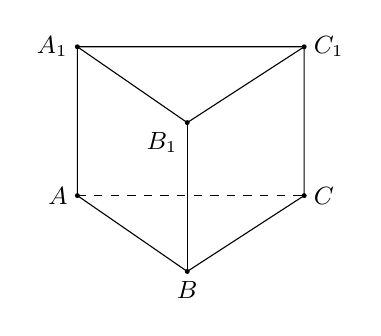
\begin{tikzpicture}[>=stealth, scale=0.9, font=\small]
  \coordinate (A)  at (0,1.45);
  \coordinate (C)  at (3.20,1.45);
  \coordinate (B)  at (1.55,0.38);
  \coordinate (A1) at (0,3.55);
  \coordinate (B1) at (1.55,2.48);
  \coordinate (C1) at (3.20,3.55);
  % 可见棱
  \draw (A1) -- (C1) -- (C) -- (B) -- (A) -- (A1);
  \draw (A1) -- (B1) -- (C1);
  \draw (B1) -- (B);
  % 不可见棱
  \draw[dashed] (A) -- (C);
  % 顶点
  \fill (A) circle (1pt) node[left] {$A$};
  \fill (B) circle (1pt) node[below] {$B$};
  \fill (C) circle (1pt) node[right] {$C$};
  \fill (A1) circle (1pt) node[left] {$A_1$};
  \fill (B1) circle (1pt) node[below left] {$B_1$};
  \fill (C1) circle (1pt) node[right] {$C_1$};
\end{tikzpicture}
\end{center}
\nopagebreak[4]
\Needspace{4\baselineskip}
\textbf{解析}

\Needspace{5\baselineskip}
正三棱柱的侧棱 $CC_1\parallel AA_1$，故异面直线 $BC_1$ 与 $AA_1$ 所成的角就是
\nopagebreak[4]
\[\angle BC_1C=\frac\pi6.\]
\Needspace{5\baselineskip}
又 $CC_1\perp$ 底面 $ABC$，所以 $CC_1\perp BC$，$\triangle BCC_1$ 在 $C$ 处为直角。于是
\nopagebreak[4]
\[BC=CC_1\tan\angle BC_1C=6\cdot\tan\frac\pi6=6\cdot\frac{\sqrt3}{3}=2\sqrt3.\]
\Needspace{5\baselineskip}
底面是边长为 $2\sqrt3$ 的正三角形，面积为
\nopagebreak[4]
\[S_{\triangle ABC}=\frac{\sqrt3}{4}BC^2=\frac{\sqrt3}{4}\cdot12=3\sqrt3.\]
\Needspace{5\baselineskip}
故三棱柱体积
\nopagebreak[4]
\[V=S_{\triangle ABC}\cdot AA_1=3\sqrt3\cdot6=18\sqrt3.\]

\gkanswer{答案：$18\sqrt3$。$BC=6\tan\dfrac\pi6=2\sqrt3$，$S_{\triangle ABC}=3\sqrt3$，$V=3\sqrt3\times6$。}

\end{answer}
\begin{answer}
\gksolhead{26}{}

\textbf{题目}（本题满分 7 分）：

如图，某校有一块形如直角三角形 $ABC$ 的空地，其中 $\angle B$ 为直角，$AB$ 长 $40$ 米，$BC$ 长 $50$ 米，现欲在此空地上建造一间健身房，其占地形状为矩形，且 $B$ 为矩形的一个顶点，求该健身房的最大占地面积。
\nopagebreak[4]
\begin{center}% 2013 年春季上海卷第 26 题：直角三角形 ABC 与内接矩形 EBFP
% 图中 AB=4、BC=5 仅为示意比例；矩形 E-B-F-P 的顶点 P 在斜边 AC 上。
\begin{tikzpicture}[>=stealth, scale=1.0, font=\small]
  \coordinate (B) at (0,0);
  \coordinate (C) at (5.0,0);
  \coordinate (A) at (0,4.0);
  \coordinate (E) at (0,2.0);
  \coordinate (F) at (2.5,0);
  \coordinate (P) at (2.5,2.0);
  \draw (A) -- (B) -- (C) -- cycle;
  \draw (E) -- (B) -- (F) -- (P) -- cycle;
  % 直角标记
  \draw (0,0.32) -- (0.32,0.32) -- (0.32,0);
  % 顶点
  \fill (A) circle (1pt) node[above] {$A$};
  \fill (B) circle (1pt) node[below left] {$B$};
  \fill (C) circle (1pt) node[below right] {$C$};
  \fill (E) circle (1pt) node[left] {$E$};
  \fill (F) circle (1pt) node[below] {$F$};
  \fill (P) circle (1pt) node[right] {$P$};
\end{tikzpicture}
\end{center}
\nopagebreak[4]
\Needspace{4\baselineskip}
\textbf{解析}

\Needspace{5\baselineskip}
设矩形为 $EBFP$，其中 $E$ 在 $AB$ 上，$F$ 在 $BC$ 上，$P$ 在斜边 $AC$ 上，$B$ 为直角顶点。设
\nopagebreak[4]
\[FP=x\quad(0<x<40).\]
\Needspace{5\baselineskip}
由于 $FP\parallel AB$，$\triangle CFP\sim\triangle CBA$，故
\nopagebreak[4]
\[\frac{FP}{BA}=\frac{CF}{CB},\]
\Needspace{5\baselineskip}
即
\nopagebreak[4]
\[\frac{x}{40}=\frac{CF}{50},\]
\Needspace{5\baselineskip}
得
\nopagebreak[4]
\[CF=\frac54x,\qquad BF=50-\frac54x.\]
\Needspace{5\baselineskip}
矩形面积
\nopagebreak[4]
\[y=BF\cdot FP=\left(50-\frac54x\right)x
=-\frac54x^2+50x
=-\frac54(x-20)^2+500.\]
\Needspace{5\baselineskip}
因为 $-\dfrac54<0$，所以
\nopagebreak[4]
\[y\leqslant500,\]
当且仅当 $x=20$（此时 $BF=25$，在允许范围内）时取等号。

故健身房的最大占地面积为 $500$ 平方米。

\gkanswer{答案：$500$ 平方米。设 $FP=x$，$BF=50-\dfrac54x$，面积 $=-\dfrac54(x-20)^2+500$。}

\end{answer}
\begin{answer}
\gksolhead{27}{}

\textbf{题目}（本题满分 8 分）：

已知数列 $\{a_n\}$ 的前 $n$ 项和为 $S_n=-n^2+n$，数列 $\{b_n\}$ 满足 $b_n=2^{a_n}$，求 $\displaystyle\lim_{n\to\infty}(b_1+b_2+\cdots+b_n)$。

\Needspace{4\baselineskip}
\textbf{解析}

\Needspace{5\baselineskip}
当 $n\geqslant2$ 时，
\nopagebreak[4]
\[a_n=S_n-S_{n-1}=(-n^2+n)-\left[-(n-1)^2+(n-1)\right].\]
\Needspace{5\baselineskip}
展开化简：
\nopagebreak[4]
\[a_n=-n^2+n+(n-1)^2-(n-1)=-2n+2.\]
\Needspace{5\baselineskip}
又
\nopagebreak[4]
\[a_1=S_1=-1+1=0,\]
\Needspace{5\baselineskip}
与 $-2\cdot1+2=0$ 一致，故对一切 $n\in\mathbf N^*$，
\nopagebreak[4]
\[a_n=-2n+2.\]
\Needspace{5\baselineskip}
于是
\nopagebreak[4]
\[b_n=2^{a_n}=2^{-2n+2}=4^{1-n}=\left(\frac14\right)^{n-1}.\]
\Needspace{5\baselineskip}
数列 $\{b_n\}$ 是首项为 $1$、公比为 $\dfrac14$ 的无穷等比数列，故
\nopagebreak[4]
\[\lim_{n\to\infty}(b_1+b_2+\cdots+b_n)
=\frac{1}{1-\frac14}
=\frac43.\]

\gkanswer{答案：$\dfrac43$。$a_n=-2n+2$，$b_n=\left(\dfrac14\right)^{n-1}$，无穷等比级数和为 $\dfrac{1}{1-\frac14}$。}

\end{answer}
\begin{answer}
\gksolhead{28}{}

\textbf{题目}（本题满分 13 分）：

本题共有 $2$ 个小题，第 $1$ 小题满分 $4$ 分，第 $2$ 小题满分 $9$ 分。

已知椭圆 $C$ 的两个焦点分别为 $F_1(-1,0)$、$F_2(1,0)$，短轴的两个端点分别为 $B_1$、$B_2$。

（1） 若 $\triangle F_1B_1B_2$ 为等边三角形，求椭圆 $C$ 的方程；

（2） 若椭圆 $C$ 的短轴长为 $2$，过点 $F_2$ 的直线 $l$ 与椭圆 $C$ 相交于 $P$、$Q$ 两点，且 $\overrightarrow{F_1P}\perp\overrightarrow{F_1Q}$，求直线 $l$ 的方程。

\Needspace{4\baselineskip}
\textbf{解析}

\Needspace{5\baselineskip}
\textbf{（1）} 设椭圆方程为
\nopagebreak[4]
\[\frac{x^2}{a^2}+\frac{y^2}{b^2}=1\quad(a>b>0).\]
\Needspace{5\baselineskip}
焦距 $2c=2$，故 $c=1$，且
\nopagebreak[4]
\[a^2-b^2=c^2=1.\]
\Needspace{5\baselineskip}
短轴端点为 $B_1(0,b)$、$B_2(0,-b)$，故
\nopagebreak[4]
\[|B_1B_2|=2b.\]
\Needspace{5\baselineskip}
又 $|F_1B_1|=\sqrt{c^2+b^2}=a$。等边三角形要求
\nopagebreak[4]
\[2b=a.\]
\Needspace{5\baselineskip}
与 $a^2-b^2=1$ 联立：
\nopagebreak[4]
\[4b^2-b^2=1,\qquad b^2=\frac13,\qquad a^2=\frac43.\]
\Needspace{5\baselineskip}
故椭圆方程为
\nopagebreak[4]
\[\frac{x^2}{4/3}+\frac{y^2}{1/3}=1,\]
\Needspace{5\baselineskip}
即
\nopagebreak[4]
\[\frac{3x^2}{4}+3y^2=1.\]

\Needspace{5\baselineskip}
\textbf{（2）} 短轴长 $2b=2$，故 $b=1$；又 $c=1$，所以
\nopagebreak[4]
\[a^2=b^2+c^2=2,\]
\Needspace{5\baselineskip}
椭圆为
\nopagebreak[4]
\[\frac{x^2}{2}+y^2=1.\]

\Needspace{5\baselineskip}
若直线 $l$ 斜率不存在，则 $l:x=1$。代入得 $y=\pm\dfrac{\sqrt2}{2}$，此时
\nopagebreak[4]
\[\overrightarrow{F_1P}\cdot\overrightarrow{F_1Q}
=(2,\tfrac{\sqrt2}{2})\cdot(2,-\tfrac{\sqrt2}{2})
=4-\frac12=\frac72\neq0,\]
不符合题意。

\Needspace{5\baselineskip}
故设 $l:y=k(x-1)$。代入椭圆方程：
\nopagebreak[4]
\[\frac{x^2}{2}+k^2(x-1)^2=1,\]
\Needspace{5\baselineskip}
整理得
\nopagebreak[4]
\[(2k^2+1)x^2-4k^2x+2(k^2-1)=0.\]
\Needspace{5\baselineskip}
设 $P(x_1,y_1)$、$Q(x_2,y_2)$，则
\nopagebreak[4]
\[x_1+x_2=\frac{4k^2}{2k^2+1},\qquad
x_1x_2=\frac{2(k^2-1)}{2k^2+1}.\]
\Needspace{5\baselineskip}
且
\nopagebreak[4]
\[\overrightarrow{F_1P}=(x_1+1,y_1),\qquad
\overrightarrow{F_1Q}=(x_2+1,y_2),\]
其中 $y_1=k(x_1-1)$，$y_2=k(x_2-1)$。

\Needspace{5\baselineskip}
由垂直条件：
\nopagebreak[4]
\[\begin{aligned}
0&=\overrightarrow{F_1P}\cdot\overrightarrow{F_1Q}\\
&=(x_1+1)(x_2+1)+k^2(x_1-1)(x_2-1)\\
&=(k^2+1)x_1x_2-(k^2-1)(x_1+x_2)+(k^2+1).
\end{aligned}\]
\Needspace{5\baselineskip}
代入韦达定理：
\nopagebreak[4]
\[\begin{aligned}
0&=\frac{(k^2+1)\cdot2(k^2-1)-4k^2(k^2-1)+(k^2+1)(2k^2+1)}{2k^2+1}\\
&=\frac{7k^2-1}{2k^2+1}.
\end{aligned}\]
\Needspace{5\baselineskip}
故
\nopagebreak[4]
\[7k^2-1=0,\qquad k^2=\frac17,\qquad k=\pm\frac{\sqrt7}{7}.\]
\Needspace{5\baselineskip}
所求直线为
\nopagebreak[4]
\[y=\pm\frac{\sqrt7}{7}(x-1),\]
\Needspace{5\baselineskip}
即
\nopagebreak[4]
\[x+\sqrt7y-1=0\quad\text{\text{或}}\quad x-\sqrt7y-1=0.\]

\gkanswer{答案（1）：$\dfrac{3x^2}{4}+3y^2=1$（即 $\dfrac{x^2}{4/3}+\dfrac{y^2}{1/3}=1$）。由 $a=2b$ 与 $a^2-b^2=1$ 得 $b^2=\dfrac13$，$a^2=\dfrac43$。}

\gkanswer{答案（2）：$x+\sqrt7y-1=0$ 或 $x-\sqrt7y-1=0$。设 $y=k(x-1)$，由 $\overrightarrow{F_1P}\cdot\overrightarrow{F_1Q}=0$ 得 $k^2=\dfrac17$。}

\end{answer}
\begin{answer}
\gksolhead{29}{}

\textbf{题目}（本题满分 12 分）：

本题共有 $2$ 个小题，第 $1$ 小题满分 $6$ 分，第 $2$ 小题满分 $6$ 分。

已知抛物线 $C:y^2=4x$ 的焦点为 $F$。

（1） 点 $A$、$P$ 满足 $\overrightarrow{AP}=-2\overrightarrow{FA}$。当点 $A$ 在抛物线 $C$ 上运动时，求动点 $P$ 的轨迹方程；

（2） 在 $x$ 轴上是否存在点 $Q$，使得点 $Q$ 关于直线 $y=2x$ 的对称点在抛物线 $C$ 上？如果存在，求所有满足条件的点 $Q$ 的坐标；如果不存在，请说明理由。

\Needspace{4\baselineskip}
\textbf{解析}

\Needspace{5\baselineskip}
\textbf{（1）} 抛物线 $y^2=4x$ 的焦点为
\nopagebreak[4]
\[F(1,0).\]
\Needspace{5\baselineskip}
设 $P(x,y)$，$A(x_A,y_A)$，则
\nopagebreak[4]
\[\overrightarrow{AP}=(x-x_A,y-y_A),\qquad
\overrightarrow{FA}=(x_A-1,y_A).\]
\Needspace{5\baselineskip}
由 $\overrightarrow{AP}=-2\overrightarrow{FA}$ 得
\nopagebreak[4]
\[\begin{cases}
x-x_A=-2(x_A-1),\\
y-y_A=-2y_A.
\end{cases}\]
\Needspace{5\baselineskip}
解得
\nopagebreak[4]
\[\begin{cases}
x_A=2-x,\\
y_A=-y.
\end{cases}\]
\Needspace{5\baselineskip}
因为 $A$ 在 $y^2=4x$ 上，所以
\nopagebreak[4]
\[y_A^2=4x_A,\]
\Needspace{5\baselineskip}
即
\nopagebreak[4]
\[(-y)^2=4(2-x).\]
\Needspace{5\baselineskip}
故动点 $P$ 的轨迹方程为
\nopagebreak[4]
\[y^2=8-4x,\]
\Needspace{5\baselineskip}
即
\nopagebreak[4]
\[x=2-\frac{y^2}{4}.\]

\textbf{（2）} 设 $Q(t,0)$，它关于直线 $y=2x$ 的对称点为 $Q'(x,y)$。

\Needspace{5\baselineskip}
直线 $y=2x$ 即 $2x-y=0$，其法向量为 $(2,-1)$。点 $Q(t,0)$ 到直线的垂足为
\nopagebreak[4]
\[Q-\frac{2t}{2^2+(-1)^2}(2,-1)
=(t,0)-\frac{2t}{5}(2,-1)
=\left(\frac t5,\frac{2t}5\right).\]
\Needspace{5\baselineskip}
故对称点
\nopagebreak[4]
\[Q'=2\left(\frac t5,\frac{2t}5\right)-(t,0)
=\left(-\frac{3t}5,\frac{4t}5\right).\]

\Needspace{5\baselineskip}
若 $Q'$ 在 $y^2=4x$ 上，则
\nopagebreak[4]
\[\left(\frac{4t}5\right)^2=4\left(-\frac{3t}5\right),\]
\Needspace{5\baselineskip}
即
\nopagebreak[4]
\[\frac{16t^2}{25}=-\frac{12t}{5}.\]
\Needspace{5\baselineskip}
两边乘以 $25$：
\nopagebreak[4]
\[16t^2=-60t,\]
\Needspace{5\baselineskip}
即
\nopagebreak[4]
\[4t^2+15t=0,\]
\Needspace{5\baselineskip}
解得
\nopagebreak[4]
\[t=0\quad\text{\text{或}}\quad t=-\frac{15}{4}.\]
\Needspace{5\baselineskip}
故存在满足条件的点
\nopagebreak[4]
\[Q(0,0)\quad\text{\text{和}}\quad Q\left(-\frac{15}{4},0\right).\]

\gkanswer{答案（1）：$y^2=8-4x$。由 $\overrightarrow{AP}=-2\overrightarrow{FA}$ 得 $x_A=2-x$，$y_A=-y$，代入 $y_A^2=4x_A$。}

\gkanswer{答案（2）：$(0,0)$ 和 $\left(-\dfrac{15}{4},0\right)$。$Q(t,0)$ 的对称点为 $\left(-\dfrac{3t}5,\dfrac{4t}5\right)$，代入 $y^2=4x$ 得 $4t^2+15t=0$。}

\end{answer}
\begin{answer}
\gksolhead{30}{}

\textbf{题目}（本题满分 13 分）：

本题共有 $2$ 个小题，第一小题满分 $4$ 分，第二小题满分 $9$ 分。

在平面直角坐标系 $xOy$ 中，点 $A$ 在 $y$ 轴正半轴上，点 $P_n$ 在 $x$ 轴上，其横坐标为 $x_n$，且 $\{x_n\}$ 是首项为 $1$、公比为 $2$ 的等比数列，记 $\angle P_nAP_{n+1}=\theta_n$，$n\in\mathbf N^*$。
\nopagebreak[4]
\begin{center}% 2013 年春季上海卷第 30 题：y 轴正半轴上的点 A 与 x 轴上的点列 P1,P2,P3,P4
% 各射线自 A 引出；P4 之后以点列省略号表示继续。
\begin{tikzpicture}[>=stealth, scale=1.0, font=\small]
  \coordinate (O) at (0,0);
  \coordinate (A) at (0,3.4);
  \coordinate (P1) at (1.05,0);
  \coordinate (P2) at (1.80,0);
  \coordinate (P3) at (2.75,0);
  \coordinate (P4) at (4.40,0);
  \draw[->] (0,0) -- (7.10,0) node[below] {$x$};
  \draw[->] (0,0) -- (0,4.05) node[left] {$y$};
  \node[below left] at (0,0) {$O$};
  \foreach \p in {P1,P2,P3,P4}{
    \draw (A) -- (\p);
    \fill (\p) circle (1.3pt);
  }
  % 点列省略号
  \fill (5.55,0) circle (0.7pt);
  \fill (5.85,0) circle (0.7pt);
  \fill (6.15,0) circle (0.7pt);
  \fill (A) circle (1.3pt) node[left] {$A$};
  \node[below] at (P1) {$P_1$};
  \node[below] at (P2) {$P_2$};
  \node[below] at (P3) {$P_3$};
  \node[below] at (P4) {$P_4$};
\end{tikzpicture}
\end{center}
\nopagebreak[4]
（1） 若 $\theta_3=\arctan\dfrac13$，求点 $A$ 的坐标；

（2） 若点 $A$ 的坐标为 $(0,8\sqrt2)$，求 $\theta_n$ 的最大值及相应 $n$ 的值。

\Needspace{4\baselineskip}
\textbf{解析}

\Needspace{5\baselineskip}
\textbf{（1）} 设 $A(0,t)$（$t>0$）。由 $\{x_n\}$ 是首项为 $1$、公比为 $2$ 的等比数列，得
\nopagebreak[4]
\[x_n=2^{n-1},\]
故 $P_n(2^{n-1},0)$，特别地 $P_3(4,0)$，$P_4(8,0)$。

\Needspace{5\baselineskip}
记 $\alpha_n=\angle OAP_n$，则
\nopagebreak[4]
\[\tan\alpha_3=\frac{4}{t},\qquad \tan\alpha_4=\frac{8}{t}.\]
\Needspace{5\baselineskip}
因为
\nopagebreak[4]
\[\theta_3=\angle P_3AP_4=\alpha_4-\alpha_3,\]
\Needspace{5\baselineskip}
所以
\nopagebreak[4]
\[\begin{aligned}
\tan\theta_3
&=\tan(\alpha_4-\alpha_3)\\
&=\frac{\frac8t-\frac4t}{1+\frac8t\cdot\frac4t}\\
&=\frac{\frac4t}{1+\frac{32}{t^2}}
=\frac{4t}{t^2+32}.
\end{aligned}\]
\Needspace{5\baselineskip}
由 $\theta_3=\arctan\dfrac13$ 得 $\tan\theta_3=\dfrac13$，于是
\nopagebreak[4]
\[\frac{4t}{t^2+32}=\frac13.\]
\Needspace{5\baselineskip}
去分母：
\nopagebreak[4]
\[12t=t^2+32,\]
\Needspace{5\baselineskip}
即
\nopagebreak[4]
\[t^2-12t+32=0,\]
\Needspace{5\baselineskip}
解得
\nopagebreak[4]
\[t=4\quad\text{\text{或}}\quad t=8.\]
故点 $A$ 的坐标为 $(0,4)$ 或 $(0,8)$。

\Needspace{5\baselineskip}
\textbf{（2）} 此时 $A(0,8\sqrt2)$。由
\nopagebreak[4]
\[\tan\angle OAP_n=\frac{x_n}{8\sqrt2}=\frac{2^{n-1}}{8\sqrt2},\]
\Needspace{5\baselineskip}
及 $\theta_n=\angle P_nAP_{n+1}=\angle OAP_{n+1}-\angle OAP_n$，得
\nopagebreak[4]
\[\begin{aligned}
\tan\theta_n
&=\frac{\frac{2^n}{8\sqrt2}-\frac{2^{n-1}}{8\sqrt2}}
{1+\frac{2^n}{8\sqrt2}\cdot\frac{2^{n-1}}{8\sqrt2}}\\
&=\frac{\frac{2^{n-1}}{8\sqrt2}}{1+\frac{2^{2n-1}}{128}}
=\frac{2^{n-1}}{8\sqrt2+2^{2n-1}\cdot8\sqrt2/128}\\
&=\frac{1}{\frac{16\sqrt2}{2^n}+\frac{2^n}{8\sqrt2}}.
\end{aligned}\]
\Needspace{5\baselineskip}
两项均为正，且乘积为
\nopagebreak[4]
\[\frac{16\sqrt2}{2^n}\cdot\frac{2^n}{8\sqrt2}=2,\]
\Needspace{5\baselineskip}
由基本不等式
\nopagebreak[4]
\[\frac{16\sqrt2}{2^n}+\frac{2^n}{8\sqrt2}\geqslant2\sqrt2,\]
\Needspace{5\baselineskip}
故
\nopagebreak[4]
\[\tan\theta_n\leqslant\frac{1}{2\sqrt2}=\frac{\sqrt2}{4}.\]
\Needspace{5\baselineskip}
等号成立当且仅当
\nopagebreak[4]
\[\frac{16\sqrt2}{2^n}=\frac{2^n}{8\sqrt2},\]
\Needspace{5\baselineskip}
即
\nopagebreak[4]
\[2^{2n}=256,\qquad n=4.\]
\Needspace{5\baselineskip}
又 $A$ 在 $y$ 轴正半轴、$P_n$ 在 $x$ 轴正半轴，射线 $AP_n$ 与 $AP_{n+1}$ 均在第四象限方向，故
\nopagebreak[4]
\[0<\theta_n<\frac\pi2.\]
\Needspace{5\baselineskip}
而 $y=\tan x$ 在 $\left(0,\dfrac\pi2\right)$ 上单调递增，所以当 $n=4$ 时 $\theta_n$ 取得最大值
\nopagebreak[4]
\[\arctan\frac{\sqrt2}{4}.\]

\gkanswer{答案（1）：$(0,4)$ 或 $(0,8)$。$\tan\theta_3=\dfrac{4t}{t^2+32}=\dfrac13$，解得 $t=4$ 或 $t=8$。}

\gkanswer{答案（2）：$n=4$ 时 $\theta_n$ 最大，最大值为 $\arctan\dfrac{\sqrt2}{4}$。$\tan\theta_n=\dfrac{1}{\frac{16\sqrt2}{2^n}+\frac{2^n}{8\sqrt2}}\leqslant\dfrac{\sqrt2}{4}$，等号在 $n=4$ 时成立。}

\end{answer}
\begin{answer}
\gksolhead{31}{}

\textbf{题目}（本题满分 18 分）：

本题共有 $3$ 个小题，第 $1$ 小题满分 $5$ 分，第 $2$ 小题满分 $7$ 分，第 $3$ 小题满分 $6$ 分。

已知真命题：“函数 $y=f(x)$ 的图像关于点 $P(a,b)$ 成中心对称图形”的充要条件为“函数 $y=f(x+a)-b$ 是奇函数”。

（1） 将函数 $g(x)=x^3-3x^2$ 的图像向左平移 $1$ 个单位，再向上平移 $2$ 个单位，求此时图像对应的函数解析式，并利用题设中的真命题求函数 $g(x)$ 图像对称中心的坐标；

（2） 求函数 $h(x)=\log_2\dfrac{2x}{4-x}$ 图像对称中心的坐标；

（3） 已知命题：“函数 $y=f(x)$ 的图像关于某直线成轴对称图像”的充要条件为“存在实数 $a$ 和 $b$，使得函数 $y=f(x+a)-b$ 是偶函数”。判断该命题的真假。如果是真命题，请给予证明；如果是假命题，请说明理由，并类比题设的真命题对它进行修改，使之成为真命题（不必证明）。

\Needspace{4\baselineskip}
\textbf{解析}

\Needspace{5\baselineskip}
\textbf{（1）} 将 $g(x)=x^3-3x^2$ 的图像向左平移 $1$ 个单位、再向上平移 $2$ 个单位，所得解析式为
\nopagebreak[4]
\[y=(x+1)^3-3(x+1)^2+2.\]
\Needspace{5\baselineskip}
展开：
\nopagebreak[4]
\[\begin{aligned}
y&=x^3+3x^2+3x+1-3x^2-6x-3+2\\
&=x^3-3x.
\end{aligned}\]
函数 $y=x^3-3x$ 满足 $(-x)^3-3(-x)=-(x^3-3x)$，是奇函数。

\Needspace{5\baselineskip}
根据题设真命题，$g$ 的图像关于点 $(a,b)$ 中心对称，当且仅当
\nopagebreak[4]
\[g(x+a)-b\]
\Needspace{5\baselineskip}
为奇函数。这里
\nopagebreak[4]
\[g(x+1)+2=x^3-3x\]
\Needspace{5\baselineskip}
为奇函数，对应 $a=1$，$b=-2$（因为 $g(x+a)-b=g(x+1)+2$）。故 $g(x)$ 图像对称中心的坐标为
\nopagebreak[4]
\[(1,-2).\]

\Needspace{5\baselineskip}
\textbf{（2）} 设 $h(x)=\log_2\dfrac{2x}{4-x}$ 的对称中心为 $P(a,b)$。令
\nopagebreak[4]
\[F(x)=h(x+a)-b
=\log_2\frac{2(x+a)}{4-(x+a)}-b
=\log_2\frac{2x+2a}{4-a-x}-b.\]
\Needspace{5\baselineskip}
$F(x)$ 为奇函数，其定义域必须关于原点对称。真数大于零：
\nopagebreak[4]
\[\frac{2x+2a}{4-a-x}>0,\]
\Needspace{5\baselineskip}
其解集的端点由分子、分母的零点
\nopagebreak[4]
\[x=-a,\qquad x=4-a\]
\Needspace{5\baselineskip}
给出，故定义域为以 $\dfrac{(-a)+(4-a)}2=2-a$ 为中点的区间。要关于原点对称，必须
\nopagebreak[4]
\[2-a=0,\qquad a=2.\]
\Needspace{5\baselineskip}
此时
\nopagebreak[4]
\[F(x)=\log_2\frac{2x+4}{2-x}-b,\qquad x\in(-2,2).\]
\Needspace{5\baselineskip}
由 $F(-x)+F(x)=0$ 对一切 $x\in(-2,2)$ 成立：
\nopagebreak[4]
\[\log_2\frac{4-2x}{2+x}+\log_2\frac{4+2x}{2-x}-2b=0.\]
\Needspace{5\baselineskip}
两对数真数之积为
\nopagebreak[4]
\[\frac{(4-2x)(4+2x)}{(2+x)(2-x)}
=\frac{16-4x^2}{4-x^2}=4,\]
\Needspace{5\baselineskip}
故
\nopagebreak[4]
\[\log_2 4-2b=0,\]
\Needspace{5\baselineskip}
即
\nopagebreak[4]
\[2-2b=0,\qquad b=1.\]
\Needspace{5\baselineskip}
所以 $h(x)$ 图像对称中心的坐标为
\nopagebreak[4]
\[(2,1).\]

\textbf{（3）} 该命题是假命题。

取 $f(x)=x$。直线 $y=x$ 关于直线 $y=-x$ 对称：点 $(u,u)$ 关于 $y=-x$ 的对称点为 $(-u,-u)$，仍在直线 $y=x$ 上，故 $f(x)=x$ 的图像关于直线 $y=-x$ 成轴对称图形。

\Needspace{5\baselineskip}
但对任意实数 $a$、$b$，
\nopagebreak[4]
\[f(x+a)-b=x+a-b,\]
这是一次函数，图像为斜率 $1$ 的直线，不关于 $y$ 轴对称，故不是偶函数。因此命题的充分性不成立（“关于某直线成轴对称”推不出“存在 $a,b$ 使 $f(x+a)-b$ 为偶函数”）。

类比题设真命题，修改后的真命题为：

“函数 $y=f(x)$ 的图像关于直线 $x=a$ 成轴对称图像”的充要条件是“函数 $y=f(x+a)$ 是偶函数”。

\gkanswer{答案（1）：$y=x^3-3x$；对称中心为 $(1,-2)$。平移后为奇函数，对应 $a=1$，$b=-2$。}

\gkanswer{答案（2）：$(2,1)$。由定义域关于原点对称得 $a=2$，再由 $F(-x)+F(x)=0$ 得 $b=1$。}

\gkanswer{答案（3）：假命题。反例 $f(x)=x$；修改为“函数 $y=f(x)$ 的图像关于直线 $x=a$ 成轴对称图像”的充要条件是“函数 $y=f(x+a)$ 是偶函数”。}

\end{answer}